\section{RAE 2822}
Flow over the RAE 2822 airfoil is discussed in this section. Experimental data is obtained from the AGARD advisory report 138~\cite{agard}. The report provides results for a large set of conditions, however only two of these are run in this report: cases 3 and 9. The free-stream conditions and the solvers ran are tabulated in~\Cref{tab:raecases}. \Cref{fig:raesynmesh,fig:raenxmesh} show the mesh used in syn3D and NX Flow respectively. The average $y^+$ of the first layer for both grids is around 1. 
\begin{table}
    \centering
    \caption{Case specifications for the RAE 2822 and which code they were run with.}
    \label{tab:raecases}    
    \begin{tabular}{@{}l ccc cc@{}}
    \toprule
    Case & $M_\infty$ & $\Rey \times 10^{6}$ & $\alpha$ (\degc) & syn3D & NX Flow \\
    \midrule
    3 & 0.6 & 6.3 & 2.57 & Yes & Yes \\
    9 & 0.730 & 6.5 & 3.19 & Yes & No \\
    \bottomrule
    \end{tabular}
\end{table}
\begin{figure}
    \centering
    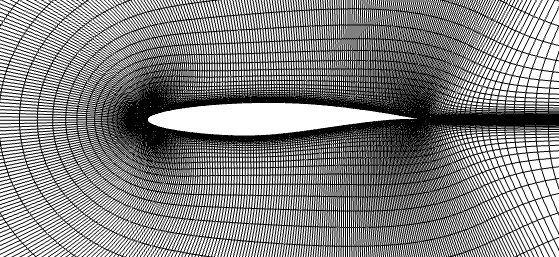
\includegraphics[width=0.7\textwidth]{figs/rae/synrae}
    \caption{Close-up of the syn3D mesh for the RAE 2822 case.}
    \label{fig:raesynmesh}
\end{figure}
\begin{figure}
    \centering
    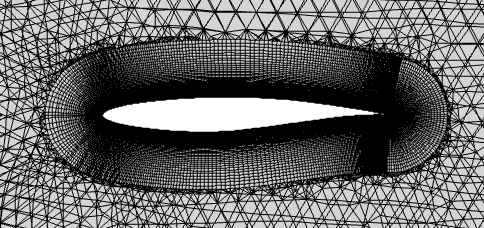
\includegraphics[width=0.7\textwidth]{figs/rae/nxrae}
    \caption{Close-up of the NX Flow mesh for the RAE 2822 case.}
    \label{fig:raenxmesh}
\end{figure}
%
%
\subsection{Case 3}
%
%
\Cref{fig:raecp3} compares the pressure coefficient over the airfoil between NX Flow, syn3D and the experimental data. \Cref{fig:raecf3} compares the skin friction coefficient only for syn3D and NX Flow, since no experimental data is available. It can be seen that syn3D over-predicts the suction on the upper surface at the leading edge, whereas NX Flow under-predicts it. The skin friction coefficient distribution is different between syn3D and NX Flow, but similar trends can be observed.

\Cref{tab:raecase3} tabulates the lift and drag coefficients. Syn3D slightly over-predicts both the lift and drag, whereas NX Flow under-predicts the lift and significantly over-predicts drag, as it did for the NACA0012 case. 
\begin{table}
    \centering
    \caption{RAE 2822 case 3 (syn3D \& NX Flow): Comparison of drag and lift coefficients with experimental data.}
    \label{tab:raecase3}
    \begin{tabular}{@{}lcc@{}}
        \toprule
        Source & $C_L$ & $C_D$ \\
        \midrule
        Experimental & 0.5220 & 0.0101 \\
        syn3D & 0.5907 & 0.0115 \\ 
        NX Flow & 0.4865 & 0.0348 \\
         \bottomrule
    \end{tabular}
\end{table}
\begin{figure}
    \centering
    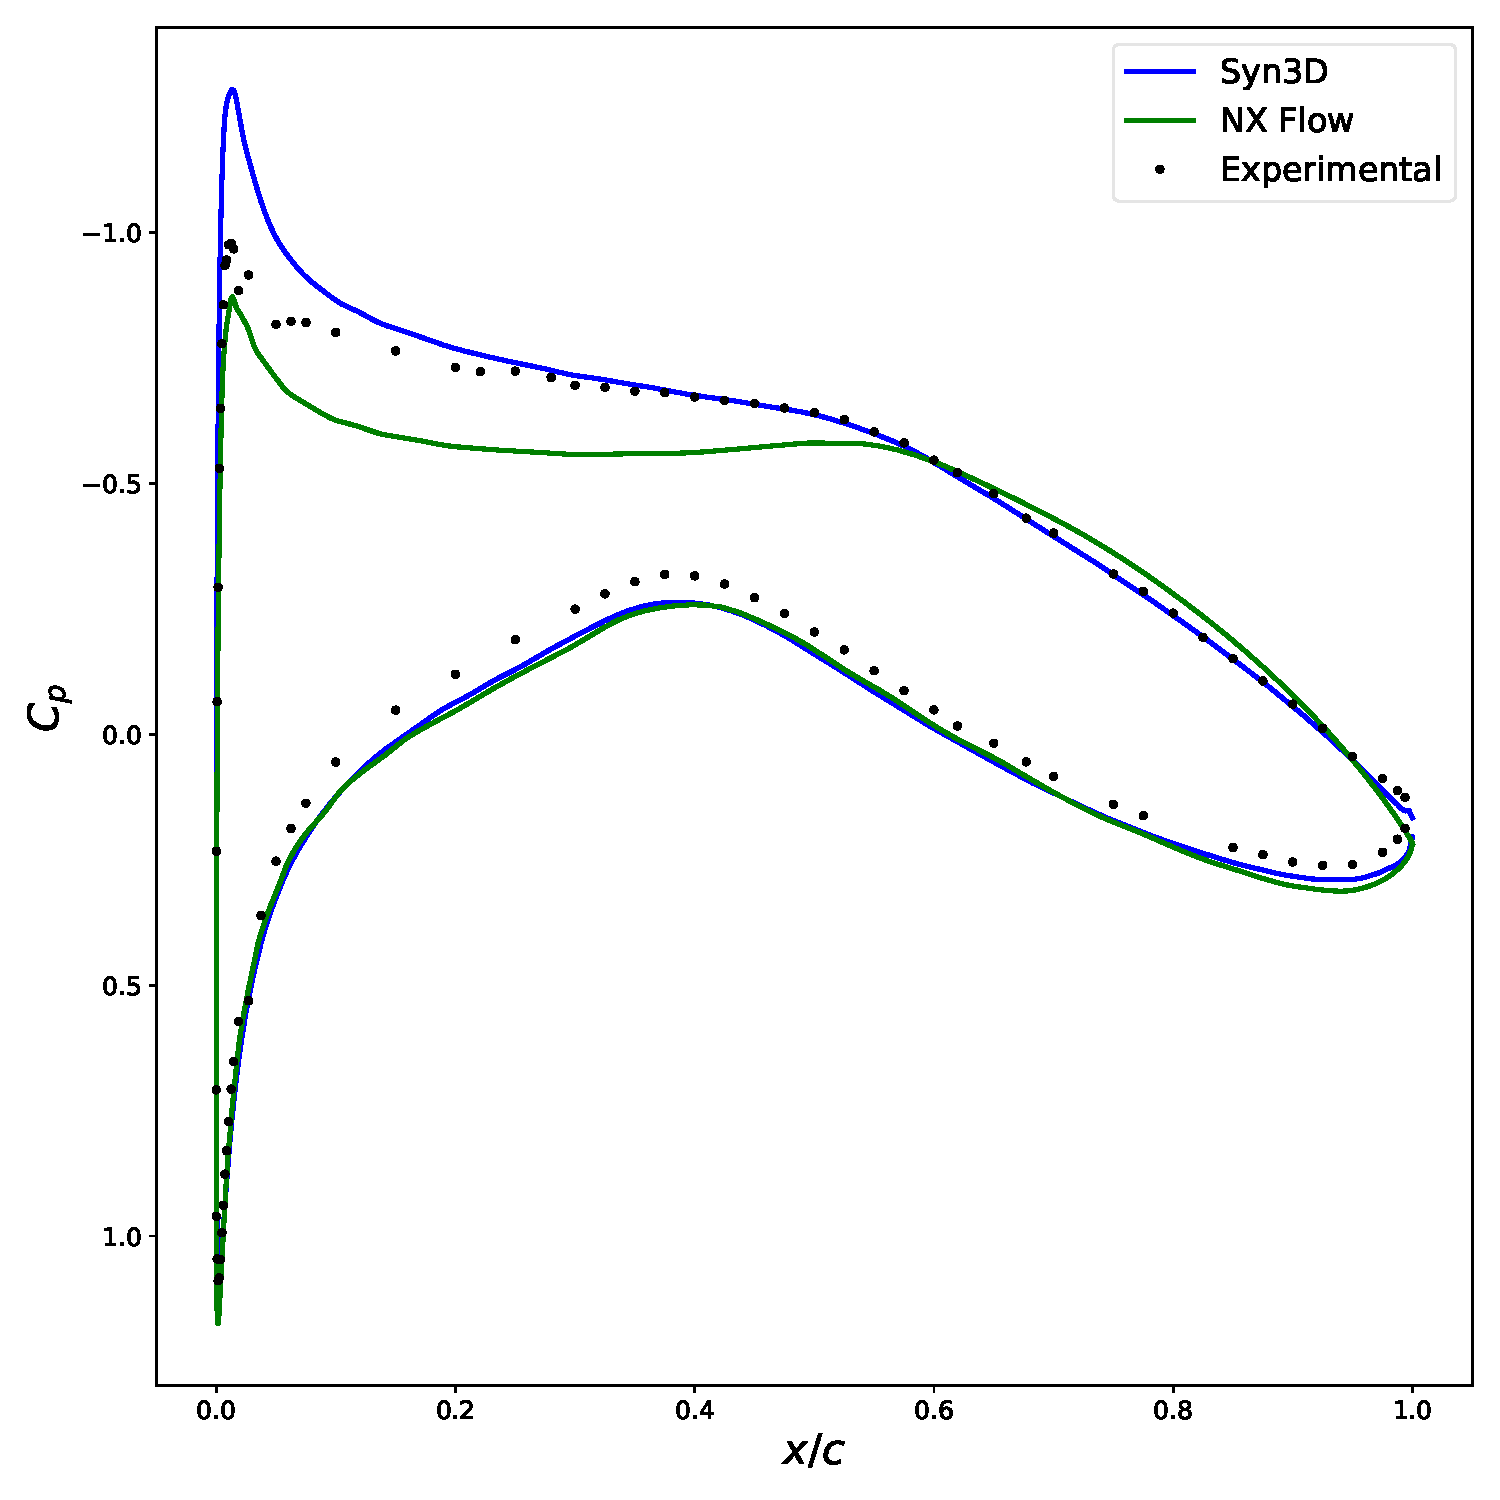
\includegraphics[width=0.7\textwidth]{figs/rae/cp_case3}
    \caption{RAE 2822 case 3 (syn3D \& NX Flow): Coefficient of pressure along the airfoil.}
    \label{fig:raecp3}
\end{figure}
\begin{figure}
    \centering
    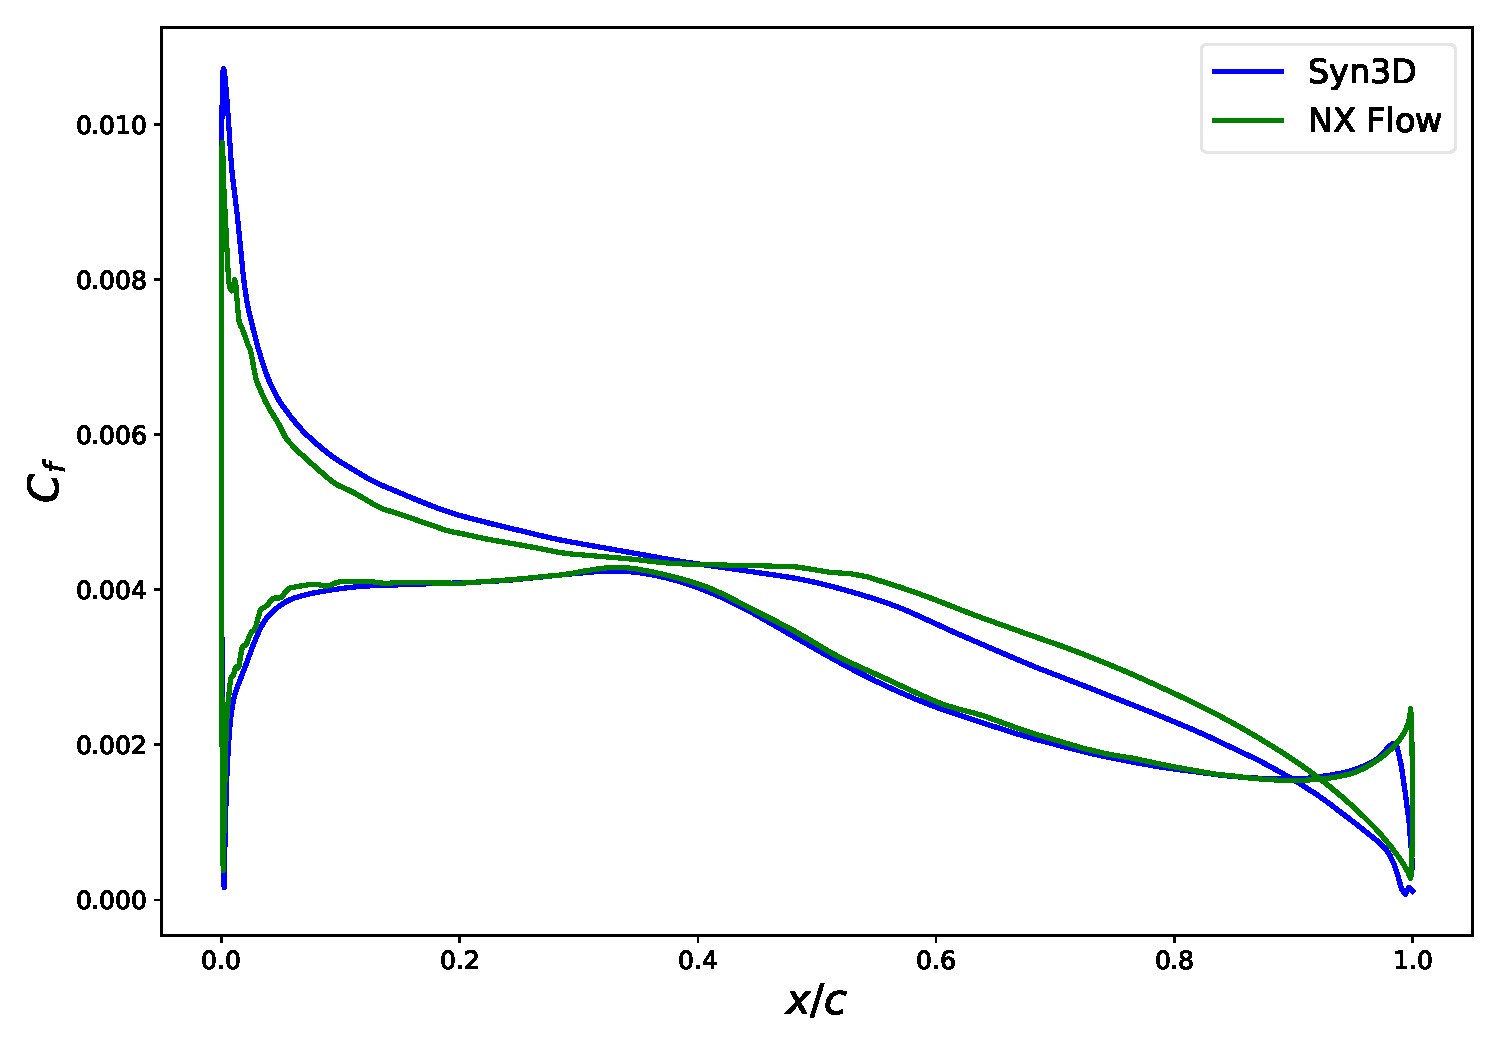
\includegraphics[width=0.7\textwidth]{figs/rae/cf_case3}
    \caption{RAE 2822 case 3 (syn3D \& NX Flow) : Coefficient of skin friction along the airfoil.}
    \label{fig:raecf3}
\end{figure}

\subsection{Case 9}
\Cref{fig:raecp9} compares the pressure coefficient over the airfoil between syn3D and experimental data. A shock can be observed on the upper surface, at around half of the chord length. This shock is well captured by syn3D and the location approximately matches that of the experimental data. \Cref{fig:raecf9} shows the skin friction coefficient on the upper surface. A shock can be observed in this plot as well, at around half the chord length.  

\Cref{tab:raecase9} tabulates the lift and drag coefficients. Once again, syn3D slightly over-predicts both the lift and drag. 
\begin{table}
    \centering
    \caption{RAE 2822 case 9 (syn3D): Comparison of drag and lift coefficients with experimental data.}
    \label{tab:raecase9}
    \begin{tabular}{@{}lcc@{}}
        \toprule
        Source & $C_L$ & $C_D$ \\
        \midrule
        Experimental & 0.8030 & 0.0168 \\
        syn3D & 0.8186 & 0.0225 \\ 
         \bottomrule
    \end{tabular}
\end{table}
\begin{figure}
    \centering
    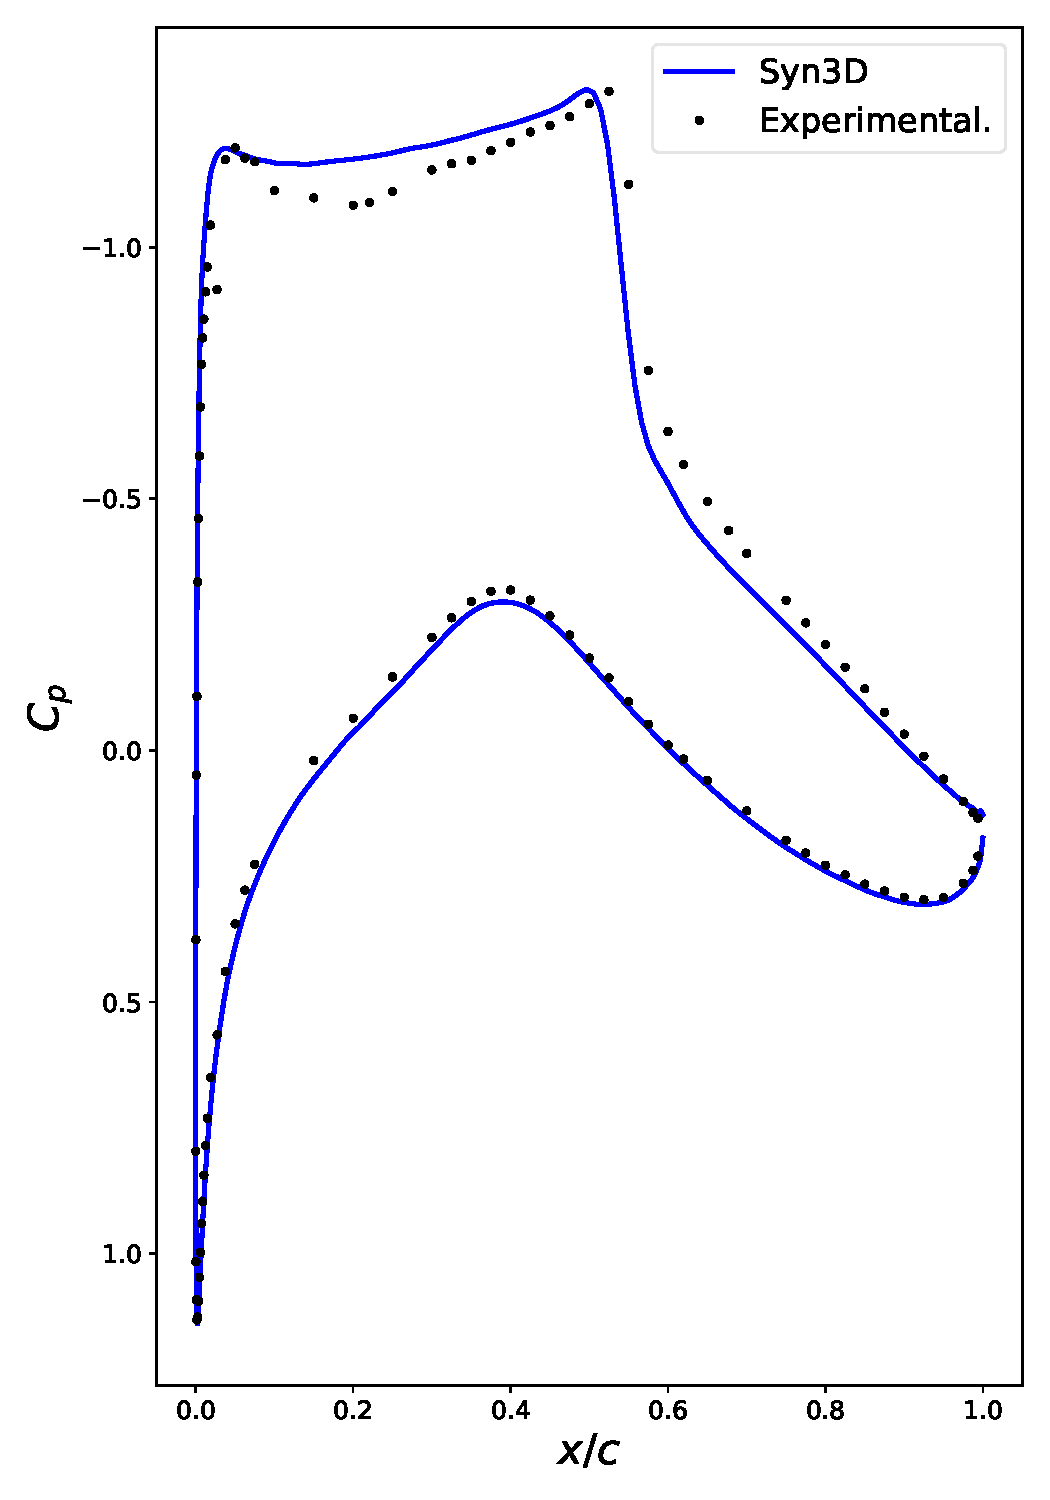
\includegraphics[width=0.7\textwidth]{figs/rae/cp_case9}
    \caption{RAE 2822 case 9 (syn3D) : Coefficient of pressure along the airfoil.}
    \label{fig:raecp9}
\end{figure}
\begin{figure}
    \centering
    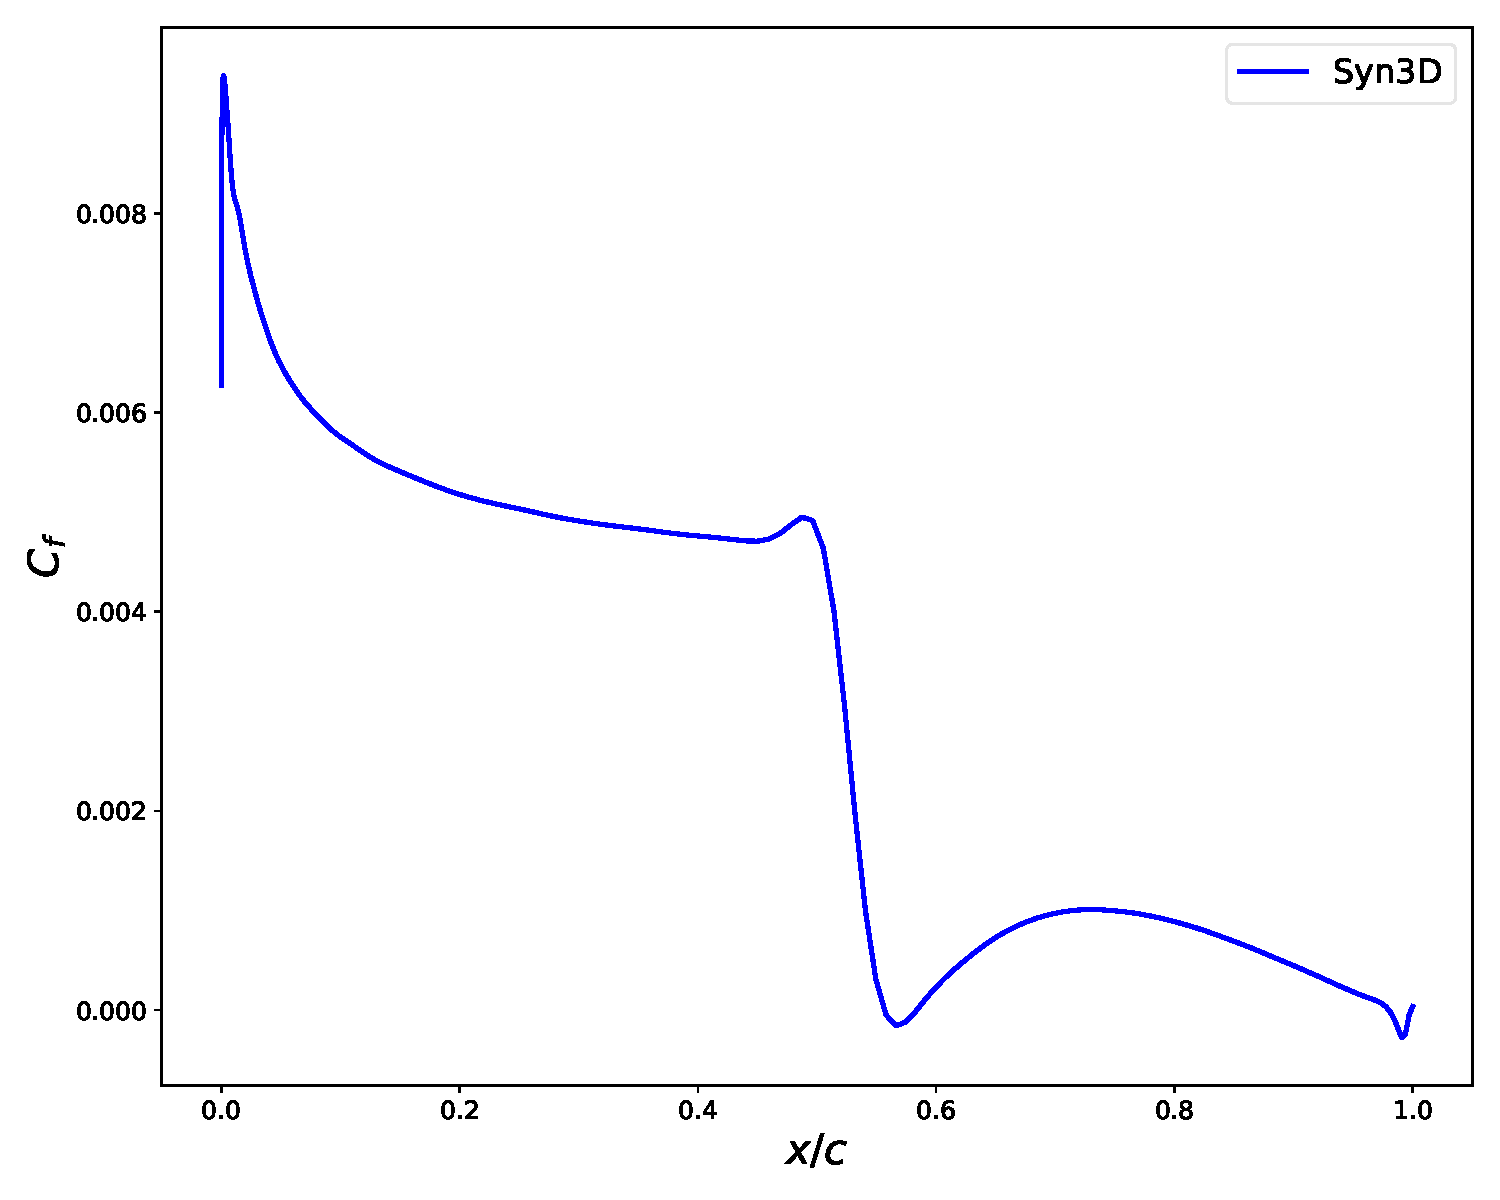
\includegraphics[width=0.7\textwidth]{figs/rae/cf_case9}
    \caption{RAE 2822 case 9 (syn3D) : Coefficient of skin friction along the upper surface of the airfoil.}
    \label{fig:raecf9}
\end{figure}